
\chapter{Framework Architecture}
\label{ch:architecture}
\section{Used Technologies}
\label{sec:technologies}

\subsection{3D FPS Game Engine}

%TA SEKCJA MNIE DEMOTYWUJE
%MNIEJ BOLAŁO PISANIE MOTYWACJI
%MIMO CZASU JAKI TRZEBA BYŁO NA NIĄ POŚWIĘCIĆ

%Nad ta sekcja warto jeszcze popracowac. Troche wiecej daloby sie tutaj napisac, np. jak zostalo ocenione code complexity i brand recognition. W wielu miejscach brakuje tutaj logicznego przeplywu mysli i sekcja jest dosc chaotyczna.

\begin{figure}
\centering
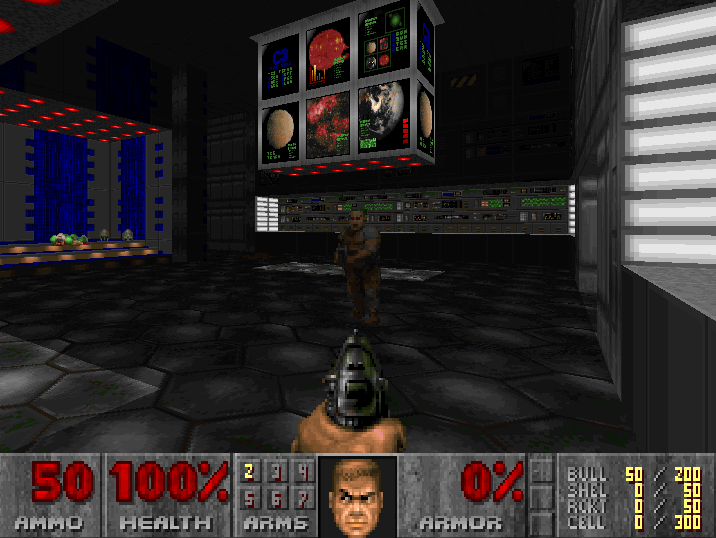
\includegraphics[scale=0.5]{doom.png}
\caption{Screenshot of Doom}
\label{fig:doom}
\end{figure}

VIZIA Environment was build around FPS game Doom. 
The environment uses  modernized version of Doom's original engine --- ZDoom~\cite{zdoom-main}. 
Screenshot from the game is shown in Figure~\ref{fig:doom}.
Doom was chosen out of 6 other recognizable FPS games considered: 

\begin{itemize}
\item Quake III Arena 
\item Doom 3
\item Half-Life 2 
\item Unreal Tournament 2004
\item Unreal Tournament
\item Cube
\end{itemize}
The comparison between them is shown in Table~\ref{tab:engines}.
% <--
Some of the criteria had to be subjective (System requirements, Code complexity), because they were based on analysis of game engine's code in the context of internal architecture, easiness of modification and performance. 
As brand recognition was treated a number (in millions) of Google results of 20.10.2016 for phrases containing only the brand name e.g., `doom' for Doom and Doom 3, `unreal tournament' for Unreal Tournament 2004 and Unreal Tournament etc.
Game was considered as able to generate small resolution image if it is possible to set resolution to smaller than 640x480.
Selecting the game was done by discarding those not meeting requirements deemed necessary.
% >--

\begin{table}[]
\centering
\caption{Overview of 3D FPS games considered as base of VIZIA environment}
\label{tab:engines}
\begin{tabular}{|p{2cm}||p{1.3cm}|p{1.3cm}|p{1.3cm}|p{1.3cm}|p{1.3cm}|p{1.3cm}|p{1.3cm}|}
\hline
Game                      & Quake III: Arena \cite{quake1}~\cite{quake2} & Doom \cite{doomreq}~\cite{zdoom}~\cite{zdoom-wiki}  & Doom 3 \cite{d3req}~\cite{idtech4}    & Half-Life 2 \cite{half2}~\cite{source} & Unreal Tournament 2004 \cite{ut04rqe}~\cite{ue2} & Unreal Tournament \cite{ue4req}~\cite{ue4faq} & Cube~\cite{cube}        \\ \hline
Game Engine               & ioquake3         & zdoom & id tech 4 & Source      & Unreal Engine 2        & Unreal Engine 4   & Cube Engine \\ \hline
Release year               & 1999             & 1993  & 2003      & 2004        & 2004                   & --\footnotemark              & 2001        \\ \hline
Open Source               & \OK              & \OK   & \OK       &             &                        & \OK               & \OK         \\ \hline
License                   & GPLv2            & GPL   & GPLv3     & Closed      & Closed                 & Custom            & ZLIB        \\ \hline
Language                  & C                & C++   & C++       & C++         & C++                    & C++               & C++         \\ \hline
DirectX                   &                  &       &           & \OK         &                        & \OK               &             \\ \hline
OpenGL                    & \OK              & \OK\footnotemark   & \OK       & \OK         & \OK                    & \OK               & \OK         \\ \hline
Software Render           &                  & \OK   &           &             &                        &                   &             \\ \hline
Windows                   & \OK              & \OK   & \OK       & \OK         & \OK                    & \OK               & \OK         \\ \hline
Linux                     & \OK              & \OK   &           & \OK         & \OK                    & \OK               & \OK         \\ \hline
Mac OS                    & \OK              & \OK   & \OK       & \OK         & \OK                    & \OK               &             \\ \hline
Scripting                 &                  & \OK   &           & \OK         & \OK                    & \OK               & \OK         \\ \hline
Custom assets             & \OK              & \OK   & \OK       & \OK         & \OK                    & \OK               & \OK         \\ \hline
Map editor                & \OK              & \OK   & \OK       & \OK         & \OK                    & \OK               & \OK         \\ \hline
Multiplayer               & \OK              & \OK   &           &             & \OK                    & \OK               & \OK         \\ \hline
Engine access             & Code             & Code  & Code      & SDK         & SDK                    & Code               & Code        \\ \hline
Small resolutions         & \OK              & \OK   & \OK       & \OK         & \OK                    & \OK               & \OK         \\ \hline
Screen buffor access      & \OK              & \OK   & \OK       &             &                        & \OK               & \OK         \\ \hline
System requirements       & Low              & Low   & Medium    & Medium      & Medium                 & High              & Low         \\ \hline
Disk space                & 70MB             & 40MB  & 2GB       & 4,5GB       & 6GB                    & \textgreater10GB\footnotemark  & 35MB        \\ \hline
Code complexity           & Medium           & Medium& High      & NA          & NA                     & High              & Low         \\ \hline
Brand recognition         & 41,1             & 99    & 99        & 36,6        & 1,2                    & 1,2               & 0,1         \\ \hline
Active community          & \OK              & \OK   & \OK       & \OK         &                        & \OK               &             \\ \hline
Free original assets      &                  &       &           &             &                        & \OK               & \OK         \\ \hline
\end{tabular}
\end{table}
\addtocounter{footnote}{-2}
\footnotetext{Unreal Tournament is in pre-alpha phase; release date is unknown.}
\stepcounter{footnote}
\footnotetext{GZDoom, ZDoom fork, is OpenGL based.}
\stepcounter{footnote}
\footnotetext{Disk requirements are yet unknown, but they will be greater than requirements of Unreal Engine 4.}
  
% <-- MOCNO ZMODYFIKOWANE, WRĘCZ NA NOWO NAPISANE
Unreal Tournament 2004 had to rejected because its engine is only accessible by Software Development Kit~(SDK) and it lacks support for controlling speed of execution and direct screen buffer access.
The game was not prepared to be heavily modified and its use in research was so far limited to server modifications.

Similar problems would have to be overcome in case of Half-Life 2, although Source engine is widely known for modding capabilities.
Although the lack of multiplayer could be solved by the use of the game Counter Strike:Source, it would introduce problems associated with the separation of game logic into client and server.

Client-server architecture was also the reason for the rejection of Quake III: Arena.
Despite wide recognition and active community, even access to the screen buffer and the possibility to modify the code could not overcome the lack of support for scripting.

Lack of scripting also concerned Doom 3. 
It had to be ignored not only for this reason, but also because of its complexity, Windows-only tools and OS-dependent rendering mechanisms.
Although its source code has been re lased, it does not have united community, so there are several rarely updated versions of its sources.%FIXME

Community activity is also a problem in case of Cube, as its last update was in August 2005~\cite{cube}.
However low complexity and highly intuitive map editor would make it a good choice, but its recognizably is so low that it had to be taken out of consideration. 

In case of Unreal Tournament there are no problems with recognition or lack of capabilities.%FIXME
Despite active community and access to source code it was out of question, because of its very high system requirements.

% >--



% <-- NAJGORSZA CZĘŚĆ FIXME
Doom met most of the given requirements and allowed to implement features that would be barely achievable in other games e.g., off-screen rendering and reward computation.
The game is highly recognizable and offers support for all needed platforms.
It was also designed to work in 320x240 resolution and despite the fact that modern implementations allow bigger resolutions, it still utilizes same low resolution textures and a rendering algorithm which makes it perfect for generating small (320x240 or smaller) visual input data for AI algorithms.
In addition its source code analysis showed that access to game logic should be easy, as its code is not object-oriented.

Unique Doom's feature is software renderer. Because of that it could be used without desktop environment (e.g., remotely over ssh) and accessing screen buffer would not require transferring it from graphics card.
% >--

\subsection{Operating System}

% <--
Development was focused on providing full functionality for Linux taking into account the compatibility of code with Windows and Mac OS.
However, on systems other than Linux VIZIA Environment has not been thoroughly tested, so support for them is limited.

% >--
% NIE MAM POMYSŁU CO MOŻNA WIĘCEJ NAPISAĆ. NIE JESTEM TEŻ PRZEKONANY CO DO OBECNOŚCI TEGO PARAGRAFU W "WYKORZYSTYWANYCH TECHNOLOGIACH". SZCZEGÓLNIE PRZY INFORMACJACH O MAC OS (OSX?) W DALSZEJ CZĘŚCI PRACY I PRZEMILCZANYM W ZASADZIE WINDOWSIE.

\subsection{Game Controller and API}


The basic module for control over Doom --- game controller --- was written in C++ with usage of Boost library.
It allowed to use Boost::interprocess library in both ZDoom and game controller, as ZDoom was written in C++.
% <--
It also made connecting game controller and game easier than it would be using low level language on the engine side and high level language for the controller.
% >--
Experimental Boost::process library was used for control over Doom process.


Above the controller, a higher layer of abstraction was implemented defining Application Programming Interface for intelligent agents modules.
API was also developed in C++, which allowed to provide bindings to Python and Java, with possibility to add another languages e.g., Lua, Julia.


Python API was considered as the main way of controlling VIZIA Environment by users.
Bindings were prepared by using Boost::python library.
This language is one of the most popular in data science~\cite{ds_lang} and widely known as it is taught at many universities all around the world~\cite{pythons_schools}.
There are many machine learning libraries for Python such as scikit-learn~\cite{scikit} or PyBrain~\cite{pybrain}.
Because of that, providing fully functional Python API was one of the biggest priorities of this project.


For Java bindings Java Native Interface (JNI) was used.


\subsection{Map Editor and Scripting}

%test environements? test scenarios? w ogole nie podoba mi sie “test scenarios”. Wole samo “scenarios” lub “game scenarios”
Creation of game scenarios has been made possible by using tools developed by Doom community for maps and scripts editing: SLADE 3~\cite{slade3} and Doom Builder 2~\cite{db2}. Those tools utilizes ACC --- a compiler for Action Code Script (ACS), language, which is supported in ZDoom engine.
This topic was discussed further in Chapter~\ref{ch:scenarios}.

\section{Architecture}\label{sec:architecture}
	\begin{figure}
			\centering
			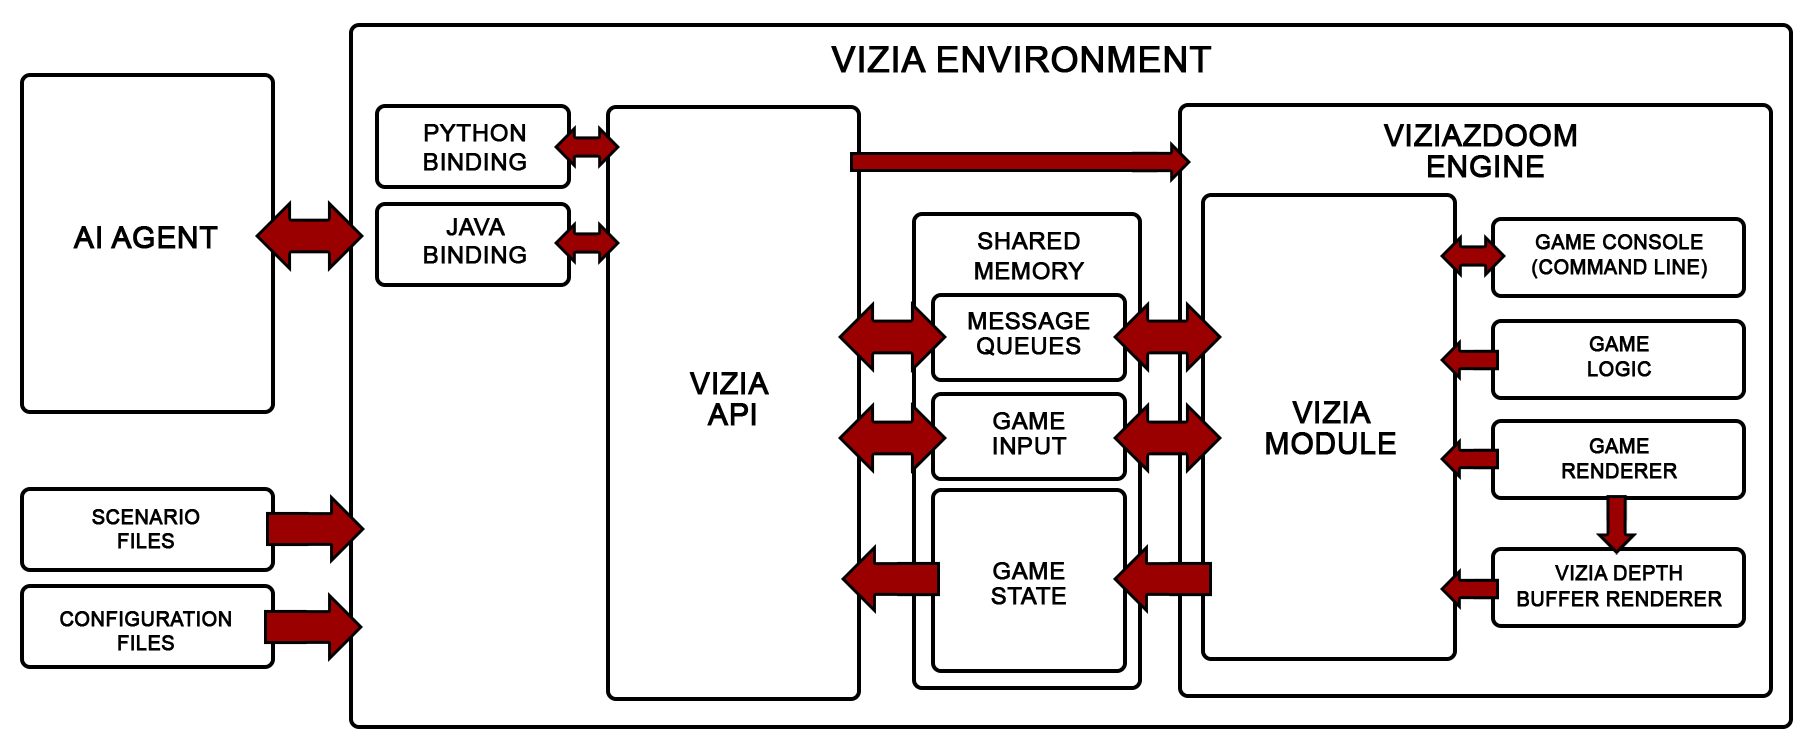
\includegraphics[scale=0.25]{architecture_diagram.png}
			\caption{Architecture of VIZIA Environment.}\label{fig:architecture_diagram}
	\end{figure}

The main components of VIZIA environament:
    \begin{itemize}
    \item VIZIA library --- which provides a DoomGame API that allows user to configure, launch and play the game in several flow control modes.
    \item VIZIAZDoom --- modified ZDoom engine with a VIZIA module to communicate with a DoomGame object, control the game flow and adding additional rendering modes. It can act as a process under the control of the DoomGame object, Dome engine used for testing in Doom editors or as standalone process.
    \item Python and Java bindings --- allowing the use of the DoomGame API in these languages.
    \end{itemize}


\subsection{The separate API and game processes}\label{sec:architecture_separate_processes}

When the API user initiates the processing, the DoomGame object creates a second thread that starts VIZIAZDoom process with the appropriate settings and supervises it. From this point the API and the game communicate using only a shared memory.


\subsection{Shared memory to communicate}\label{sec:architecture_shared_memory}

During initialization set of spaces is created in the shared memory, which includes:
    \begin{itemize}
    \item A pair of message queues to control the processing flow and sending commands to the game.
    \item A shared memory area to exchange information about game input status. Both the API process and the game process reads and writes to shared memory.
    \item Shared memory areas where the game provides state of the game. These are the values of the variables necessary to control the game's processing, values of the variables available for AI agent and a copy of the game's screen. The game process saves to the memory, the process of API support.
    \end{itemize}
All shared memory spaces have unique names for each DoomGame object, which allows the coexistence of multiple instances on one machine.


\subsection{VIZIA module inside VIZIAZDoom}\label{sec:architecture_inside_viziazdoom}

VIZIA module inside the engine initializes the shared memory to exchange information with this instance of the game. Then controls the flow of the game depending on the processing mode, and received messages and determines the following processing steps:

    \begin{itemize}
    \item Starting processing of the next game tic.
    \item Transmitting commands from the message queue to the game console.
    \item Sending input information from shared memory to the game console.
    \item Processing of events that the game window received since the last tic.
    \item Rendering the current frame.
    \item Updating the information about the current game state in the shared memory.
    \end{itemize}

\subsection{Control modes}\label{sec:architecture_modes}

The DoomGame API implements four control modes:
    
    \begin{itemize}
    \item Synchronous player
    \item Synchronous spectator
    \item Asynchronous player
    \item Asynchronous spectator
    \end{itemize}
    
    \subsubsection{Synchronous player mode}\label{sec:architecture_player_mode}
    
        \begin{figure}
			    \centering
			    
\includegraphics[scale=0.25]{player_mode_diagram.png}
			    \caption{Processing flow in synchronous player mode.}\label{fig:player_mode_diagram}
	    \end{figure}
        
	    Synchronous player mode provides synchronous communication between the process that uses the API and the game process. It allows AI agent to make actions as a player. 
	    
	    In this mode, the API and the game processes communicates every tic and are waiting for each other. The game process waits until the API sends a message requesting processing of the next tic and optional update. The game process, after receiving the message, sends input information (AI agent's action) to the game console, process next game tic, and if update was requested renders the current frame and updates the information about the current game state in the shared memory. After this, the game process sends a message about completing request and starts waiting for the message processing of the next tic. The process that uses the API waits for the message about completing request.
	    
	    This mode is designed for the singleplayer mode, multiplayer mode is not supported. For more details see Section~\ref{sec::architecture_solution_multi}.

    \subsubsection{Synchronous spectator mode}\label{sec:architecture_spectator_mode}

	    \begin{figure}
			    \centering
			    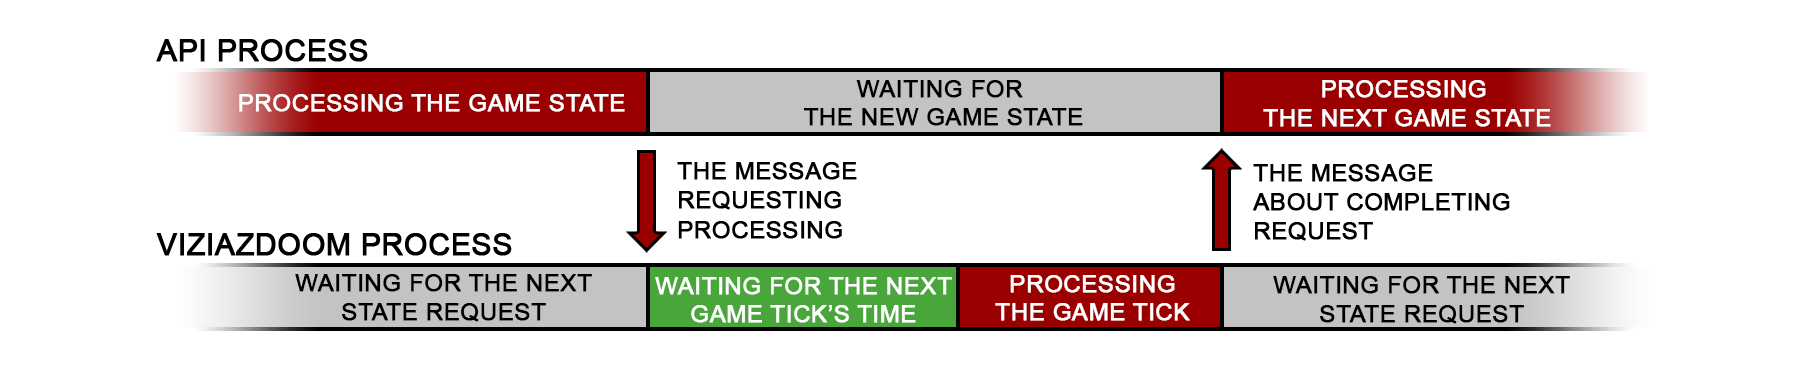
\includegraphics[scale=0.25]{spectator_mode_diagram.png}
			    \caption{Processing flow in synchronous spectator mode.}\label{fig:spectator_mode_diagram}
	    \end{figure}
	    
	    Synchronous spectator mode provides synchronous communication and allows AI agent to observe a human player's actions. 
	    
	    In this mode, the processes communicates every tic and are waiting for each other. The game process waits until the API sends a message requesting processing of the next tic and optional update. The game process, after receiving the message, process the window input events that have taken place since the two last update requests (last human player's action), updates the input information in the shared memory, process next game tic and if update was requested renders the current frame and updates the information about the current game state in the shared memory. After this, the game process sends a message about completing request and starts waiting for the message processing of the next tic. The process that uses the API waits for the message about completing request.

        Before processing of the next game tic the delay may be introduced in order to ensure the maximum processing speed of 35 tics per second (designed Doom ticrate).
        
        Similar to the synchronous player mode, this mode does not support multiplayer mode.

    \subsubsection{Asynchronous player mode}\label{sec:architecture_async_player_mode}

	    \begin{figure}
			    \centering
			    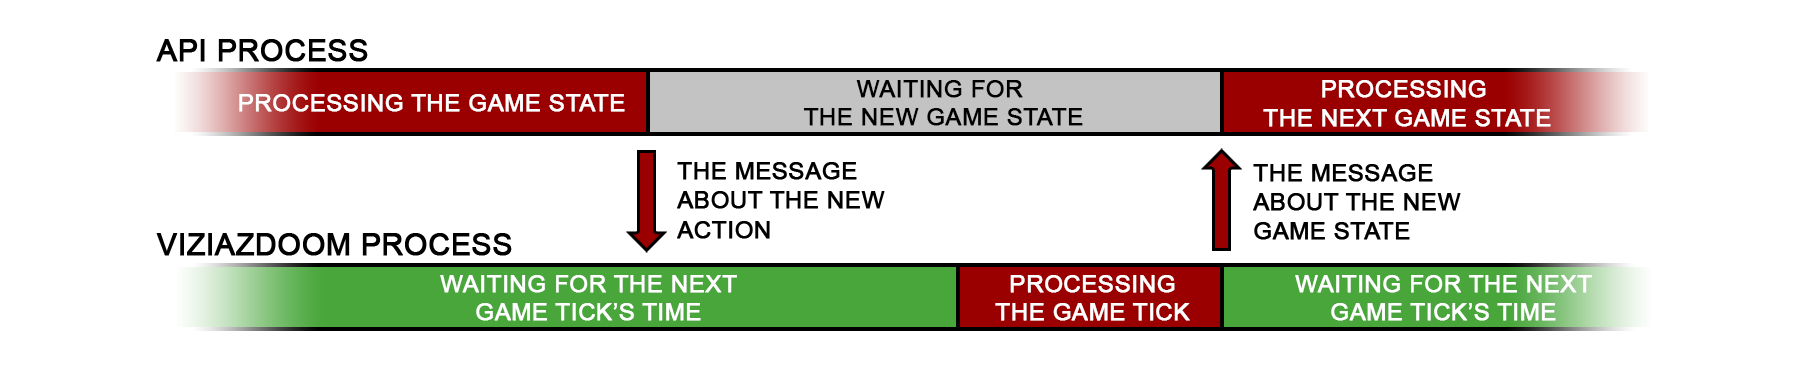
\includegraphics[scale=0.25]{async_player_mode_diagram.png}
			    \caption{Processing flow in asynchronous player mode.}\label{fig:async_player_mode_diagram}
	    \end{figure}
	    
	    Asynchronous player mode provides asynchronous communication between the process and allows AI agent to make actions as a player. 
	    
	    In this mode, the game process continuously process the game tics at a constant speed of 35 tics per second (delay is introduced between tics) without waiting for the API process. The API can send a message requesting update. Before each tic the game process checks if it received a message requesting update. After receiving such the message, it sends the input information (AI agent's action) to the game console, process next game tic, updates the information about the current game state in the shared memory, sends a message about completing request and continues processing of the game tics. The process that uses the API waits for the message about completing request.
	    
	    This mode supports both the singleplayer mode and the multiplayer mode.

    \subsubsection{Asynchronous spectator mode}\label{sec:architecture_async_spectator_mode}

	    \begin{figure}
			    \centering
			    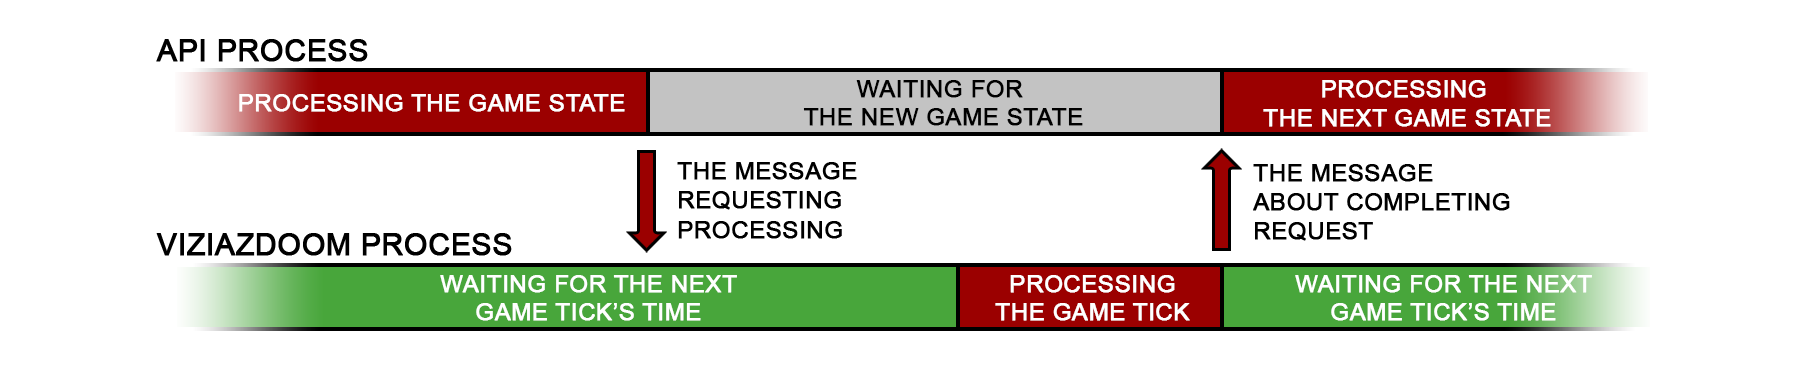
\includegraphics[scale=0.25]{async_spectator_mode_diagram.png}
			    \caption{Proce      ssing flow in asynchronous spectator mode.}\label{fig:async_spectator_mode_diagram}
	    \end{figure}
	    
	    Asynchronous spectator mode provides asynchronous communication and allows AI agent to observe a human player's actions. 
	    
	    In this mode, the game process continuously process the game tics at a constant speed of 35 tics per second without waiting for the API process. The API can send a message requesting update. Before each tic the game process checks if it received a message. After receiving such the message, it updates the input information in the shared memory (last human player's action), process next game tic, updates the information about the current game state in the shared memory, sends a message about completing request and continues processing of the game tics. The process that uses the API waits for the message about completing request.

        In this mode processing of the window input events and rendering is performed in each tic.
        
        This mode also supports both the singleplayer mode and the multiplayer mode.

\section{Other Design Decisions, Encountered problems and their Solutions}\label{sec:architecture_solutions}

\subsubsection{Why separate doom executable?}

Doom engine was designed as standalone executable. It has a different entry point for every operating system and a lot of exit points what makes it difficult to pack it inside library without making any fundamental changes to its code. In addition, this approach would not give any significant benefits. Also leaving the Doom engine as a separate executable allows to use it with Doom editors and as standalone Doom engine, which can be used for testing scenarios or human versus AI agent game in multiplayer mode.

\subsubsection{Why shared memory to communicate?}

Shared memory is the fastest way to transfer large amounts of data between processes. It allows using the data without additional copying in the process that receives it. 
Since the game process uses shared memory only on the API request and the API process is waiting for completion of this request, additional access control mechanism (such as mutexes) is not needed.

\subsubsection{Why depth buffer has been added?}

The rendering algorithm used in ZDoom engine uses binary space partitioning (BSP) trees and other rendering techniques which does not make use of depth buffer and therefore it is not generated.
% <--
Depth buffer could be find usefull for learning depth perception by agent.
In addition, information about the depth can be used to simulate the distance sensors widely used in mobile robots.  
Becouse of that, depth buffer was added to the engine as presented in Figure~\ref{fig:zbuffer}.
% >--
It is drawn only when demanded rendering mode includes it (see~\ref{subsec:screenformat}).
Depth is aproximated by texture's scaling factor and stored as 8-bit value which gives enough accuracy and allows to use it as additional color channel rather than as seperate image.

\begin{figure}
\centering
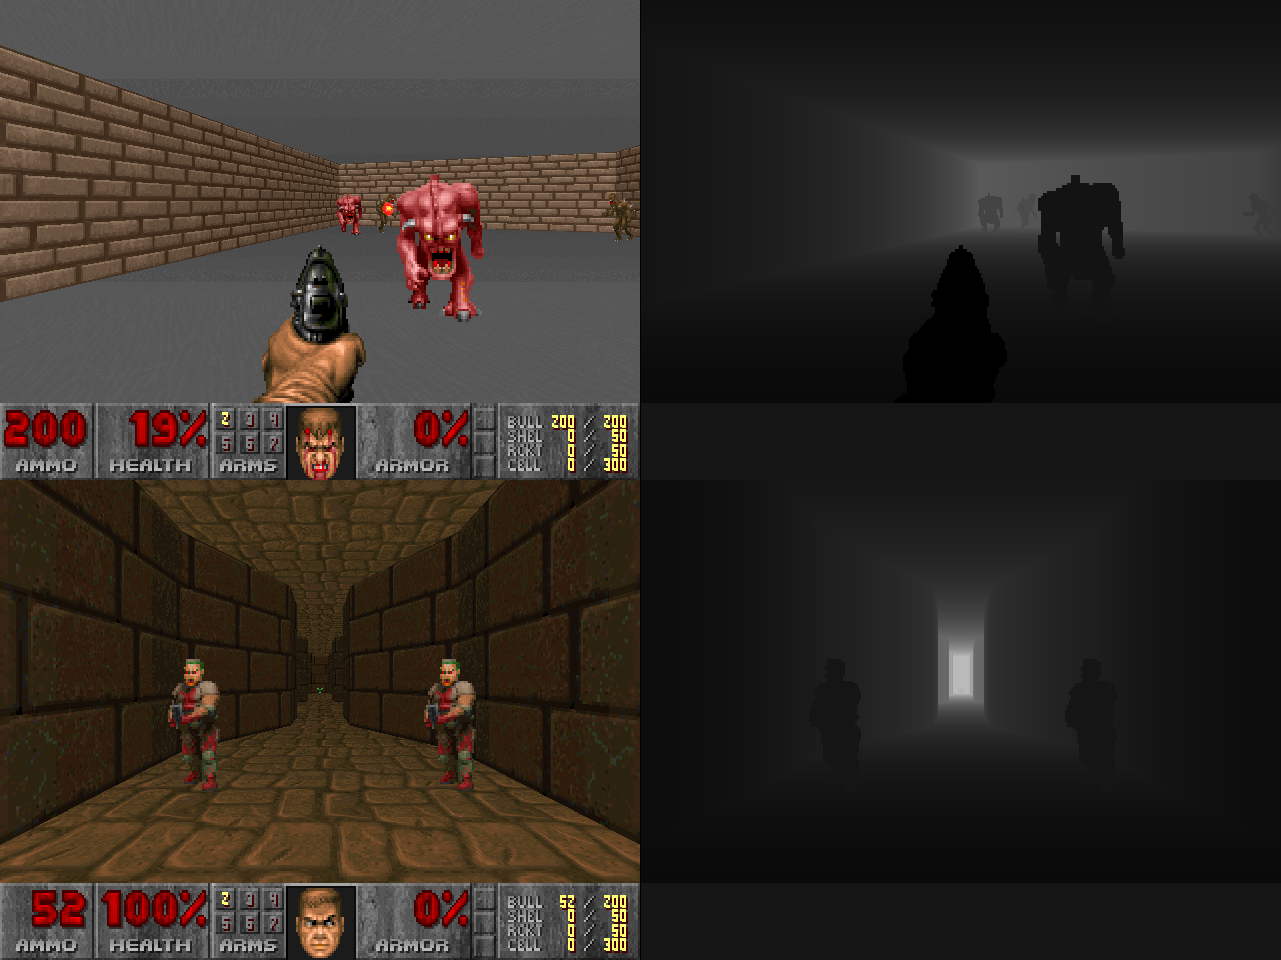
\includegraphics[scale=0.3]{zbuffer.png}
\caption{Example of implemented depth buffer}
\label{fig:zbuffer}
\end{figure}

\subsubsection{Why multiplayer is not supported in synchronous modes?}\label{sec:architecture_solution_multi}

Doom engine uses a peer-to-peer communication in multiplayer and requires synchronization between all game clients. In each tic (every 1/35th of a second) a information about input is generated and game clients should exchange it with each other. 
In synchronous modes time when next tic will be processed is unknown and may vary in different clients --- too slow or too fast processing leads to unpredictable game behaviors and errors that interrupts processing. Due to lack of time the network code has not been adapted for synchronous modes, instead it has been disabled.

\subsubsection{Why game and scenario files are separated?}

Doom engine uses different type of files for storing data and resources. (WAD and PK3 files) It allows to load main game resources from one file and many additional (scenario) resources from separate files. For more detailed information consult Zdoom Wiki Webpage\cite{zdoom-wiki}.

\section{Performance tests}\label{sec:performance}

All the Doom's processing including rendering is performed on a single processor thread. Additionally, rendering takes up most of the processing time. Therefore, the main factors affecting the processing speed is a geometry of the map, number of the actors (in-game objects like items and enemies) and the resolution. 

These factors have been taken into account during performance tests. Tests have been made in the synchronous player mode, where are no additional delays between tics and the image has been rendered in each tic.

	\subsection{Operating System and Hardware}
	
	Tests have been performed on the following specification:
	
	\begin{description}
		\item[Operating System] Linux Mint 17 x86\_64, kernel 3.13.0-24-generic
		\item[CPU] Intel Core i7-4790, 4x4GHz
	\end{description}

\subsection{Tests results}

\begin{figure}
\centering
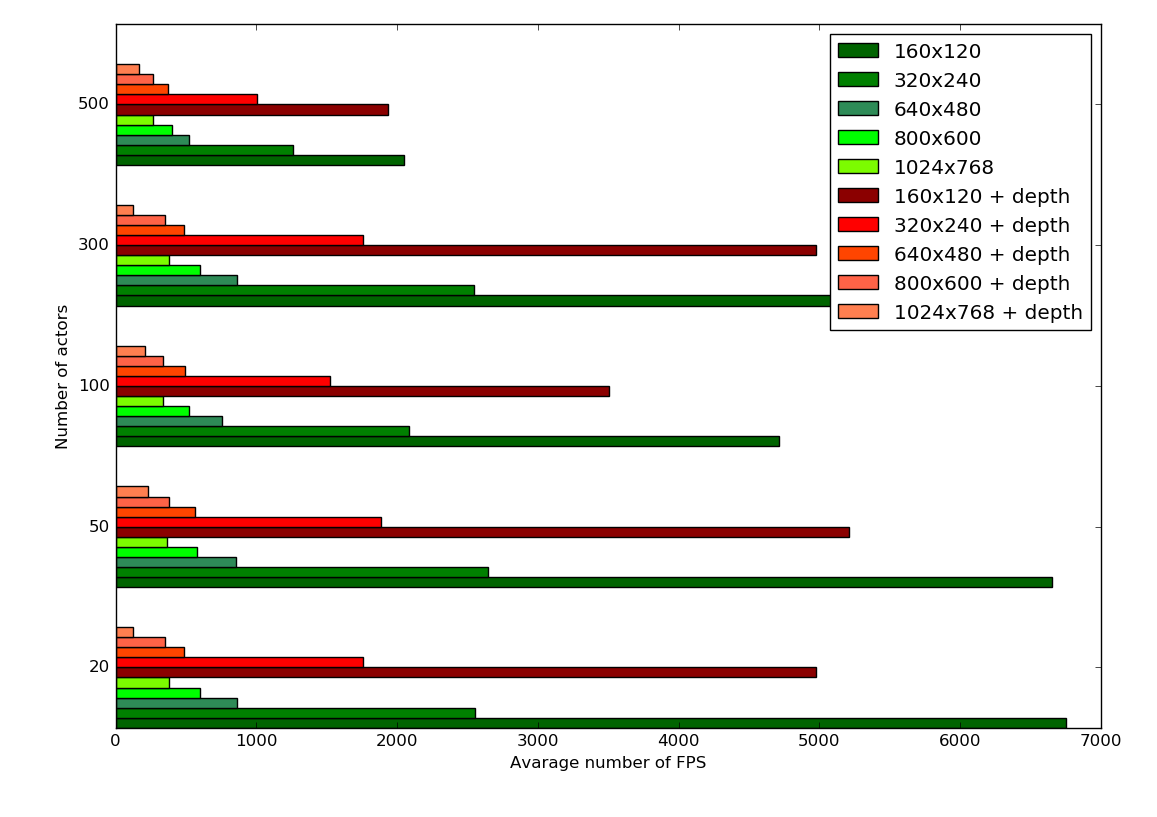
\includegraphics[scale=0.5]{result_fps.png}
\caption{Results of performance test.}
\label{fig:fps_test}
\end{figure}

Tests presented in Figure~\ref{fig:fps_test} show that the most important factor affecting performance is the rendering resolution. In case of using small resolutions, time needed to render one frame is insignificant compared to the time any reasonably good AI needs for a learning process.



